\documentclass[10pt]{article}
\usepackage{tmlr}
\usepackage{amsmath,amssymb,booktabs}
\usepackage[hidelinks]{hyperref}
\usepackage{graphicx}
\usepackage{url}
% Generated by reproduce.py. Edit the renderer or source data.
\newcommand{\FactorialRows}{%
A00 & 0 & 68.3 & 66.7 & $1.7\;[-3.3,7.0]$ \\
A00 & 1 & 60.0 & 65.0 & $-5.0\;[-15.3,6.7]$ \\
A00 & 2 & 65.0 & 61.7 & $3.3\;[0.0,10.3]$ \\
A01 & 0 & 81.7 & 55.0 & $26.7\;[1.7,48.4]$ \\
A01 & 1 & 90.0 & 61.7 & $28.3\;[9.8,48.3]$ \\
A01 & 2 & 78.3 & 45.0 & $33.3\;[11.7,54.8]$ \\
A10 & 0 & 68.3 & 30.0 & $38.3\;[15.8,57.4]$ \\
A10 & 1 & 60.0 & 36.7 & $23.3\;[6.9,38.3]$ \\
A10 & 2 & 65.0 & 40.0 & $25.0\;[3.4,43.5]$ \\
A11 & 0 & 81.7 & 41.7 & $40.0\;[16.7,62.7]$ \\
A11 & 1 & 90.0 & 28.3 & $61.7\;[38.3,83.1]$ \\
A11 & 2 & 78.3 & 38.3 & $40.0\;[20.3,58.7]$ \\
}
\newcommand{\SequenceRows}{%
A00 & 0 & 42 & 64.3 / 64.3 & 64.3 / 64.3 & 0.0 & 0.0 & 0.0 \\
A00 & 1 & 42 & 52.4 / 59.5 & 52.4 / 59.5 & -7.1 & -7.1 & -7.1 \\
A00 & 2 & 41 & 61.0 / 56.1 & 61.0 / 56.1 & 4.9 & 4.9 & 4.9 \\
A11 & 0 & 46 & 76.1 / 30.4 & 80.4 / 32.6 & 45.7 & 47.8 & 50.0 \\
A11 & 1 & 46 & 87.0 / 21.7 & 73.9 / 30.4 & 65.2 & 43.5 & 50.0 \\
A11 & 2 & 46 & 71.7 / 28.3 & 71.7 / 19.6 & 43.5 & 52.2 & 63.0 \\
}
\newcommand{\MainContrastRows}{%
0 & $45.7\;[17.2,72.1]$ & $47.8\;[26.5,69.7]$ & $50.0\;[27.9,71.8]$ \\
1 & $72.4\;[47.2,96.8]$ & $50.6\;[28.7,73.2]$ & $57.1\;[32.0,82.1]$ \\
2 & $38.6\;[14.4,61.7]$ & $47.3\;[20.3,72.3]$ & $58.2\;[28.3,84.1]$ \\
}
\newcommand{\AffineControlRows}{%
0 & $6.90\;[3.56,10.10]$ & $6.90\;[5.50,8.32]$ & 8.74 & 8.58 & 6.76 & 34/45 \\
1 & $8.16\;[4.36,11.58]$ & $8.16\;[6.65,9.70]$ & 9.11 & 9.07 & 7.45 & 35/46 \\
2 & $8.54\;[5.33,11.61]$ & $8.54\;[7.05,10.05]$ & 9.89 & 9.68 & 7.82 & 34/46 \\
}
\newcommand{\KDRows}{%
0 & 81.7 & 70.0 & $11.7\;[-1.6,25.4]$ & 15.2 & $6.39\;[3.65,8.81]$ \\
1 & 90.0 & 73.3 & $16.7\;[1.6,37.9]$ & 21.7 & $6.48\;[3.90,8.80]$ \\
2 & 78.3 & 76.7 & $1.7\;[-4.8,10.2]$ & 2.2 & $7.21\;[4.42,9.80]$ \\
}
\newcommand{\FactorialContrastRows}{%
A10$-$A00 & $36.7\;[15.5,54.8]$ & $28.3\;[13.8,42.4]$ & $21.7\;[0.0,41.3]$ \\
A11$-$A01 & $13.3\;[-1.6,30.0]$ & $33.3\;[10.0,55.2]$ & $6.7\;[-14.5,28.8]$ \\
A01$-$A00 & $25.0\;[-1.5,47.5]$ & $33.3\;[10.4,55.5]$ & $30.0\;[7.0,51.7]$ \\
A11$-$A10 & $1.7\;[-28.7,32.2]$ & $38.3\;[10.4,64.5]$ & $15.0\;[-13.2,44.0]$ \\
interaction & $-23.3\;[-47.6,3.4]$ & $5.0\;[-22.9,31.0]$ & $-15.0\;[-44.0,16.1]$ \\
}
\newcommand{\EqualFamilyRows}{%
A01$-$A00 & $23.2\;[-2.5,46.2]$ & $32.8\;[10.5,54.7]$ & $29.5\;[6.7,51.6]$ \\
A11$-$A10 & $1.1\;[-29.2,31.7]$ & $38.4\;[10.3,64.7]$ & $15.2\;[-12.7,43.8]$ \\
}
\newcommand{\ScoringChangeRows}{%
0 & $2.2\;[-25.5,25.0]$ & $2.2\;[-25.5,25.0]$ & $2.2\;[-17.4,21.7]$ & $3.6\;[-24.4,26.2]$ \\
1 & $-21.7\;[-34.0,-13.0]$ & $-21.7\;[-38.9,-5.2]$ & $-21.7\;[-39.5,-4.1]$ & $-20.8\;[-37.8,-5.1]$ \\
2 & $8.7\;[-10.9,30.4]$ & $8.7\;[-10.6,30.4]$ & $8.7\;[-6.5,23.9]$ & $9.2\;[-10.7,31.5]$ \\
}
\newcommand{\AllPairsRows}{%
A00 & 0 & 1.7 & 0.0 & 0.0 \\
A00 & 1 & -5.0 & -5.0 & -5.0 \\
A00 & 2 & 3.3 & 3.3 & 3.3 \\
A11 & 0 & 40.0 & 43.3 & 45.0 \\
A11 & 1 & 61.7 & 40.0 & 45.0 \\
A11 & 2 & 40.0 & 46.7 & 55.0 \\
}

% Generated by scripts.reanalysis_tables.py from reports/audit_reanalysis.json.
\newcommand{\ControlTestRows}{%
0 & mismatch & -1.89\,[-2.89,-0.89] & 0.009 & 0.419 & \no \\
0 & zero & -1.71\,[-2.63,-0.79] & 0.010 & 0.285 & \no \\
0 & random & 0.01\,[-2.15,2.17] & 0.993 & 0.062 & \no \\
1 & mismatch & -0.93\,[-1.75,-0.12] & 0.067 & 0.021 & \yes \\
1 & zero & -0.88\,[-1.64,-0.11] & 0.068 & 0.014 & \yes \\
1 & random & 0.67\,[-0.60,1.95] & 0.352 & 0.045 & \yes \\
2 & mismatch & -1.30\,[-2.35,-0.25] & 0.052 & 0.123 & \no \\
2 & zero & -1.09\,[-2.25,0.07] & 0.119 & 0.091 & \no \\
2 & random & 0.72\,[-0.33,1.78] & 0.236 & 0.028 & \yes \\
}
\newcommand{\ControlMeanRows}{%
0 & mismatch & 8.74\,[5.04,12.16] & 6.90\,[3.56,10.10] \\
0 & zero & 8.58\,[4.62,12.11] & 6.90\,[3.56,10.10] \\
0 & random & 6.76\,[3.90,9.92] & 6.90\,[3.56,10.10] \\
1 & mismatch & 9.11\,[5.20,12.58] & 8.16\,[4.36,11.58] \\
1 & zero & 9.07\,[5.10,12.64] & 8.16\,[4.36,11.58] \\
1 & random & 7.45\,[4.26,10.50] & 8.16\,[4.36,11.58] \\
2 & mismatch & 9.89\,[5.99,13.49] & 8.54\,[5.33,11.61] \\
2 & zero & 9.68\,[5.64,13.35] & 8.54\,[5.33,11.61] \\
2 & random & 7.82\,[4.71,10.77] & 8.54\,[5.33,11.61] \\
}
\newcommand{\ScaleRows}{%
A00 & 0 & 6.16 & 1.97 & 0.32 \\
A00 & 1 & 5.90 & 1.93 & 0.33 \\
A00 & 2 & 6.64 & 2.12 & 0.32 \\
A11 & 0 & 8.62 & 6.90 & 0.80 \\
A11 & 1 & 9.08 & 8.16 & 0.90 \\
A11 & 2 & 9.71 & 8.54 & 0.88 \\
}
\newcommand{\RankRows}{%
affine & -0.436 & $<10^{-8}$ & 180 \\
kd & +0.435 & $<10^{-8}$ & 180 \\
}
\newcommand{\MapperGapRows}{%
0 & 6.90\,[3.56,10.10] & 6.39\,[3.65,8.81] & 0.417 & 0.700 \\
1 & 8.16\,[4.36,11.58] & 6.48\,[3.90,8.80] & 0.283 & 0.733 \\
2 & 8.54\,[5.33,11.61] & 7.21\,[4.42,9.80] & 0.383 & 0.767 \\
}
\newcommand{\ExtendedScoringRows}{%
A00 & 0 & 1.7\,[-3.3,7.0] & 0.0\,[-4.8,5.1] & 0.0\,[-4.8,5.1] \\
A11 & 0 & 40.0\,[16.7,62.7] & 43.3\,[24.2,62.1] & 45.0\,[25.8,63.3] \\
A00 & 1 & -5.0\,[-15.2,6.7] & -5.0\,[-11.9,0.0] & -5.0\,[-11.9,0.0] \\
A11 & 1 & 61.7\,[38.3,83.0] & 40.0\,[21.3,58.3] & 45.0\,[23.8,66.1] \\
A00 & 2 & 3.3\,[0.0,10.3] & 3.3\,[0.0,10.3] & 3.3\,[0.0,10.3] \\
A11 & 2 & 40.0\,[20.3,58.7] & 46.7\,[24.1,68.3] & 55.0\,[29.5,78.3] \\
}
\newcommand{\ExtendedContrastRows}{%
0 & 38.3\,[13.9,61.2] & 43.3\,[23.7,62.8] & 45.0\,[25.0,64.5] \\
1 & 66.7\,[40.8,90.2] & 45.0\,[25.3,64.0] & 50.0\,[27.9,71.1] \\
2 & 36.7\,[16.1,56.5] & 43.3\,[20.0,66.0] & 51.7\,[26.2,76.3] \\
}
\newcommand{\ScoringCountRows}{%
retained\_6\_family & A00 & 0 & 42 & 6 \\
retained\_6\_family & A00 & 1 & 42 & 6 \\
retained\_6\_family & A00 & 2 & 41 & 6 \\
retained\_6\_family & A11 & 0 & 46 & 6 \\
retained\_6\_family & A11 & 1 & 46 & 6 \\
retained\_6\_family & A11 & 2 & 46 & 6 \\
f1\_f4\_all\_6\_family & A00 & 0 & 46 & 6 \\
f1\_f4\_all\_6\_family & A00 & 1 & 46 & 6 \\
f1\_f4\_all\_6\_family & A00 & 2 & 46 & 6 \\
f1\_f4\_all\_6\_family & A11 & 0 & 46 & 6 \\
f1\_f4\_all\_6\_family & A11 & 1 & 46 & 6 \\
f1\_f4\_all\_6\_family & A11 & 2 & 46 & 6 \\
all\_60\_pairs\_8\_family & A00 & 0 & 60 & 8 \\
all\_60\_pairs\_8\_family & A00 & 1 & 60 & 8 \\
all\_60\_pairs\_8\_family & A00 & 2 & 60 & 8 \\
all\_60\_pairs\_8\_family & A11 & 0 & 60 & 8 \\
all\_60\_pairs\_8\_family & A11 & 1 & 60 & 8 \\
all\_60\_pairs\_8\_family & A11 & 2 & 60 & 8 \\
}

\newcommand{\yes}{$\checkmark$}
\newcommand{\no}{--}

\title{A Benchmark Rebuild Reverses a Cross-Model KV Transfer Finding:\\
       Controlled Version Contrasts, Control Tests, and Metric Diagnostics}
\author{}
\hypersetup{pdftitle={A Benchmark Rebuild Reverses a Cross-Model KV Transfer Finding},pdfauthor={}}

\begin{document}
\maketitle

\begin{abstract}
Cross-model key--value (KV) cache handoff is evaluated on paired counterfactual benchmarks. We audit one such benchmark for Qwen3-1.7B$\to$0.6B and find 18 degenerate must-flip pairs, at least 15 groups of verbatim cross-split document overlap, and shared template skeletons between calibration and held-out data. Rebuilding the corpus reverses the apparent success of an affine mapper: its native-minus-transferred dual-correctness gap is $-5.0$ to $3.3$ percentage points in the original/original condition, versus $23.3$ to $61.7$ points in the nine other cell--seed combinations. On the rebuilt validation sets the transferred counterfactual error is no larger than the mismatched and zero-cache controls and close to the randomized-cache control, and is significantly smaller than the zero-cache control in one seed, even though dual correctness collapses to $28.3$--$41.7\%$. A pre-declared equivalence test ($\delta=2$ log-probability units) succeeds in one of three seeds, so ``indistinguishable from a zero-information control'' is not uniformly supported. We further show that counterfactual error has weak discriminative validity: its intervals overlap between the affine mapper and a distillation baseline whose dual correctness differs by $28$--$45$ points, and its rank correlation with dual correctness reverses sign between the two. Full-candidate scoring preserves the direction of the version contrast in every seed but lowers its magnitude by $21.7$ points in one seed. All estimates are exploratory (at most eight template families), cover one synthetic model pair, and do not attribute the reversal to any single defect. Single-defect interventions, a sealed test and a second model pair remain unevaluated. We release the repaired benchmark, the numeric ledger and the audit protocol.
\end{abstract}

\section{Introduction}

Cache translation lets a receiver answer a query from a document processed by a different model, without prefilling that document again. Downstream answer correctness indicates whether the transmitted cache is useful; a paired-document design can additionally ask whether the receiver's candidate scores change when a fact in the document changes. These two quantities can diverge, and diagnosing the divergence presupposes a valid document pair and a receiver that can answer under both variants.

An earlier analysis of a synthetic paired benchmark suggested that an affine KV mapper preserved dual-side correctness while changing counterfactual response scores, and it suggested a receiver-side value-consumption mechanism. We withdrew both claims after auditing the benchmark: the legacy corpus contained degenerate pairs, cross-split document overlap and overlapping template skeletons, and the uncertainty estimates effectively treated related examples as independent.

\paragraph{What this study establishes.}
We cross the original and rebuilt calibration and validation corpora for one model pair and three data seeds, giving twelve cell--seed combinations. Replacing either corpus moves the correctness gap from near zero to $23.3$--$61.7$ points. We then ask two questions the version contrast alone cannot answer. First, how does the transferred counterfactual error compare with explicit no-information controls once per-seed cluster intervals and a pre-declared equivalence margin are used? Second, does the counterfactual error actually track whether transfer is useful? We answer both from archived scores without new model runs. A third check asks whether the direction survives scoring complete candidate sequences rather than only their first token.

\paragraph{Contributions.}
(1) A defect taxonomy and audit protocol covering degenerate pairs, cross-split leakage, entity and template-skeleton overlap, and clustered bootstrap degeneracy. (2) A repaired paired benchmark (\texttt{cf\_pairs\_v2.1}) with a released numeric ledger and a CPU replay. (3) Controlled evidence that the correctness gap is sensitive to corpus version, together with control, equivalence and metric-validity diagnostics: counterfactual error does not separate a useful from a useless mapper, whereas dual correctness does. (4) A scoring-readout check showing that direction survives but magnitude does not.

\paragraph{Scope of claims.}
This is an audit of one equal-depth model pair on synthetic Chinese template data, with at most eight template families and a sealed test that remains unevaluated. We do not attribute the reversal to any single defect, do not claim a mechanism on clean data, do not claim cross-model or cross-pair generalization, and do not claim that the equivalence tests are well powered. A failed equivalence test is reported as inconclusive rather than as evidence of a deficit. The estimates are exploratory throughout.

\paragraph{Related work.}
\citet{heo2026} describe closed-form KV mapping and report substantial degradation on some model pairs. \citet{kvlingo} use distillation to train KV translators, and \citet{cachelink} study differences between reconstruction fidelity and receiver utility. \citet{cheng2026} use mismatched, zero and random caches to evaluate the role of example-specific information in relayed caches. Our experiment uses similar control ideas and focuses on a reproducible benchmark-version reversal. The use of minimally changed inputs follows contrast-set evaluation \citep{contrastsets}. The data audit addresses leakage and dependent evaluation units, concerns discussed by \citet{kapoor2023}. Our contribution is the calibration-by-validation comparison together with its control, metric and scoring diagnostics.

\section{Benchmark and audit}

\paragraph{Document pairs.}
Each example contains a question, two independently constructed documents and two answer candidates. In the four semantic slices, the edit changes the correct candidate. These slices cover direct fact substitution, inference chains, relation or negation changes, and distractors or coreference. A fifth slice (F5) uses identical candidate text as a non-flip control. A sixth (F6) changes a name and its answer label while controlling length and position. We report F6 separately and exclude both F5 and F6 from the direction-consistency analysis.

\paragraph{Corpus reconstruction.}
The archived seed-0 corpus contains 520 pairs, including 120 calibration and 60 validation pairs. The corpus audit found 18 degenerate must-flip pairs, at least 15 groups of verbatim cross-split overlap, shared entities and overlap between calibration and held-out template skeletons. The historical resampling unit was effectively the individual pair. Reconstruction made the candidates distinct where an answer change was required, separated entity pools across splits, de-duplicated examples and introduced genuinely unseen templates in the probe and held-out test. For the validation data used below, 46 pairs per version and seed are in F1--F4. The original validation sets have 4, 4 and 5 degenerate must-flip pairs. The overlap of exact document strings across calibration and validation, counting strings on either document side, is 2, 5 and 1 in the original versions. The 398 reconstructed F1--F4 examples are a corpus-wide count. Figure~\ref{fig:corpus} counts the validation-side defects and their removal.

\begin{figure}[tbp]
\centering
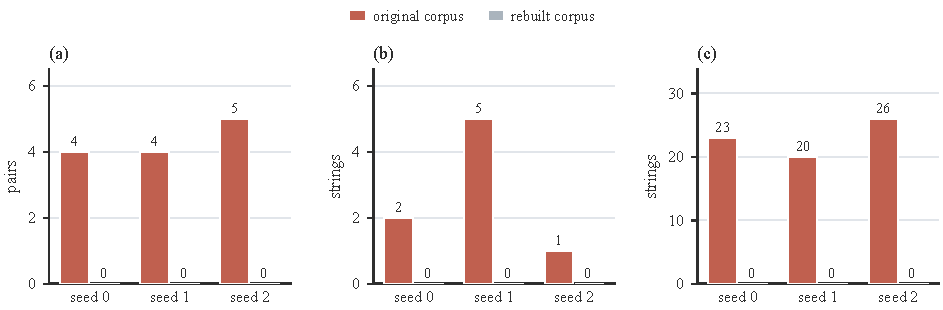
\includegraphics[width=\linewidth]{figures/fig2_corpus.pdf}
\caption{Defects in the validation split before and after the rebuild, recomputed from the released corpus files. (a) Pairs in F1--F4 whose candidates are identical although the edit is supposed to change the answer. (b) Exact document strings shared between calibration and validation. (c) Query strings shared between the two splits. Counts are per seed, and every metric is zero on the rebuilt corpus. Each panel uses its own vertical scale.}
\label{fig:corpus}
\end{figure}

Each seed identifies a generated calibration set and its corresponding validation set. The validation experiments compare corpus versions as bundles. In particular, changes made to the unseen templates in the held-out split supply no evidence for why a validation result moved. We assess each validation set in the reported experiment. The planned method endpoint on the held-out test remains unevaluated, and no single-defect intervention has been run.

\section{Evaluation}

\paragraph{Cache transfer and controls.}
We use Qwen3-1.7B as sender and Qwen3-0.6B as receiver. The two models have 28 layers with an identity layer correspondence. The receiver's weights stay frozen. The affine mapper fits a ridge regression for each layer, head and K/V component using matched sender and receiver caches from 120 calibration pairs, with $\lambda=10^{-3}$. The fit estimates about 7.40 million coefficients including intercepts, in a closed-form solve. The archived GPU runs use bfloat16 and SDPA.

The \emph{Self} condition uses the receiver's native document cache. \emph{Joint} maps both the sender keys and values. The receiver sees query tokens and, for sequence scoring, the candidate prefix. It obtains document positions from the injected cache. Identity injection checks the receiver cache path. An initial diagnostic on 80 document sides found agreement between native and identity injection, with reported minimum cosine rounding to 1.0 and first-token KL of zero. In the corpus-version experiment, mismatched, zero and randomized caches contextualize Joint's counterfactual error. The mismatch is a deterministic next-example replacement within the same validation set. We use its values from that experiment because the historical mismatch selection was different.

\paragraph{Candidate scores.}
Let $s(c;C,q)$ be the score of candidate $c$ under the query $q$ and cache $C$. The first-token proxy uses the next-token log probability of the first token of $c$. In the follow-up, $s$ is the sum of the conditional token log probabilities under teacher forcing. Candidates begin from independently initialized receiver cache branches. We concatenate independently tokenized query and candidate sequences and omit EOS. We also divide the sum by the number of candidate tokens as a length sensitivity analysis. The two candidates are ranked separately on each document side. Across all readouts we apply the historical first-candidate tie rule and credit either candidate when both are marked correct. The CPU replay verified all 720 first-token dual labels using this rule. Before harmonization, 84 F5 labels differed because the archived scorer could not credit either candidate, and six semantic labels differed because it broke exact ties towards the second candidate.

\paragraph{Metrics.}
We report the fraction of pairs answered correctly on both documents, separately for Self and Joint. Write $L$ for Self minus Joint dual correctness in percentage points. For each scoring definition, set
\begin{align}
g(C,q) &= s(A; C,q)-s(B; C,q), \\
D &= g(C(d_A),q)-g(C(d_B),q),\\
E_{\mathrm{CF}} &= |D_{\mathrm{Joint}}-D_{\mathrm{Self}}|.
\end{align}
The counterfactual error is a Joint-to-Self discrepancy. Self has zero error relative to itself. Different scoring definitions induce different error scales, so we compare correctness across readouts and keep errors within readout. Direction consistency reports agreement between the signs of the two $D$ values among F1--F4 pairs with $|D_{\mathrm{Self}}|>0.1$, together with the numerator and denominator.

\paragraph{Design and uncertainty.}
The $2\times2$ design crosses original and reconstructed calibration and validation. The first index of A00, A01, A10 and A11 denotes calibration, the second validation, and 1 denotes the reconstructed version. Three data seeds give 12 cell--seed combinations with 60 validation pairs each. Fixed-validation contrasts are paired by sample. Cross-validation contrasts resample the two sets independently. We resample template families 10,000 times and divide the total across sampled families by the number of sampled pairs on each draw. We report exploratory 95\% percentile intervals and provide pair-level or family-equal sensitivity where applicable. Validation has eight families per version, with six in the semantic scoring subset. Seeds are reported individually. The corpus-version design was versioned before its runs. The full-candidate plan was checked into Git before the reproducible scoring rerun; earlier engineering runs exist in the archive. For the control comparison below, the equivalence margin $\delta=2$ was declared in \texttt{configs/prereg/equivalence\_margin\_v2.9.yaml} before the numbers in this revision were inspected; it is an internal version-controlled protocol, not an external registration. Figure~\ref{fig:design} summarises the cache path and the four cells.

\begin{figure}[tbp]
\centering
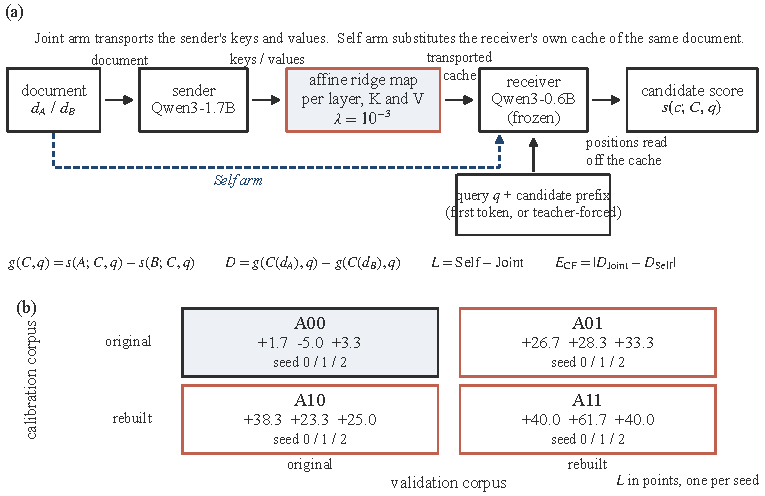
\includegraphics[width=\linewidth]{figures/fig1_design.pdf}
\caption{The cache path and the corpus-version design. Panel (a): the sender's per-layer keys and values are mapped by a per-layer, per-head affine ridge fit and injected into the frozen receiver, which then sees only the query and the candidate prefix; the dashed Self arm routes the receiver's own cache of the same document into the receiver. Panel (b): original (0) and rebuilt (1) calibration and validation corpora crossed with three data seeds, with $L$ in points for each seed; the historical A00 cell is shaded.}
\label{fig:design}
\end{figure}

\section{Results}

\subsection{Calibration and validation versions both change the result}

\begin{table}[tbp]
\centering
\caption{Corpus-version comparison on all 60 validation pairs per cell. Self and Joint are percentages. $L$ and its template-family interval are in percentage points.}
\label{tab:factorial}
\begin{tabular}{lrrrr}
\toprule
Cell & Seed & Self & Joint & $L$ [95\% interval]\\
\midrule
\FactorialRows
\bottomrule
\end{tabular}
\end{table}

Table~\ref{tab:factorial} shows near-zero gaps in the historical diagonal A00 and positive gaps from 23.3 to 61.7 points across the other nine cell--seed combinations. The six diagonal runs match their corresponding benchmark Joint error and correctness logs. On the original validation sets, replacing the calibration corpus increases $L$ by 36.7, 28.3 and 21.7 points. On the reconstructed validation sets the increases are 13.3, 33.3 and 6.7 points. These comparisons hold Self fixed and reflect how the two mappers behave on the same examples. Figure~\ref{fig:factorial} plots every cell with its interval and the two correctness levels behind each gap.

\begin{figure}[tbp]
\centering
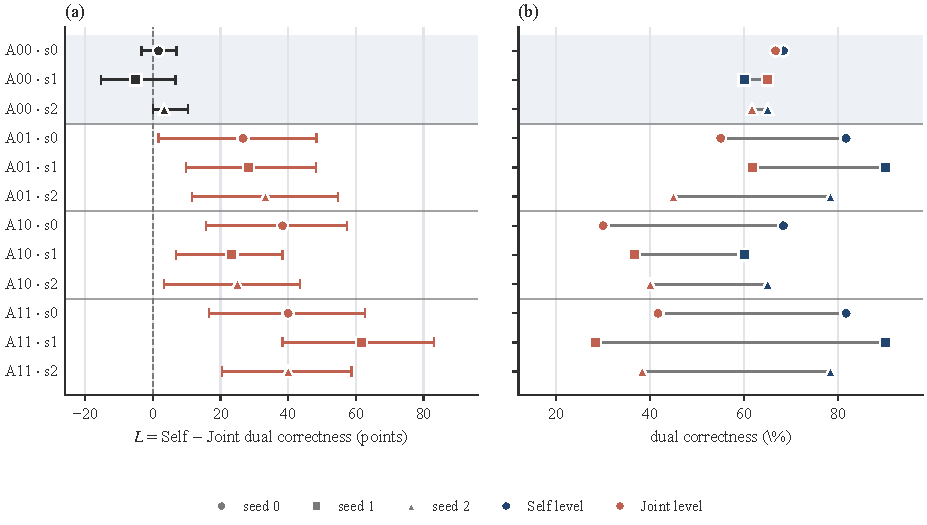
\includegraphics[width=\linewidth]{figures/fig3_factorial.pdf}
\caption{Corpus-version result. (a) $L$ in points with its exploratory template-family interval, one row per cell and seed; the historical A00 rows are shaded and the dashed line marks a zero gap. (b) The Self and transferred dual-correctness levels that produce each gap. Marker shape encodes the seed throughout; colour encodes Self/Joint in (b) and the A00/non-A00 cells in (a). Samples are compared within a row only.}
\label{fig:factorial}
\end{figure}

Replacing the validation set changes the Self reference as well. For example, with reconstructed calibration in seed~0, Joint rises from 30.0\% to 41.7\% and Self rises from 68.3\% to 81.7\%. The difference therefore widens by 1.7 points even though Joint improves. The difference of the two fixed-validation calibration contrasts is $-23.3$, $5.0$ and $-15.0$ points, with exploratory intervals covering zero in all three seeds (Appendix~\ref{app:factorial}). The result supports sensitivity to each version switch on these data. The sign of the interaction varies by seed and the design leaves effects of individual defects unresolved. Restricting to the semantic slices or removing identical candidates leaves the contrast between A00 and the other cells in place.

\subsection{Counterfactual error against no-information controls}

On reconstructed calibration and validation, Joint's first-token counterfactual error is 6.90, 8.16 and 8.54 across seeds, with family intervals in Table~\ref{tab:control-test}. Each value is no larger than the corresponding mismatched and zero-cache means and close to the randomized-cache mean; the paired family-level difference is negative for mismatch and zero in all seeds and reaches a two-sided $p=0.010$ against zero in seed~0 and $p=0.067$ in seed~1. The direction is therefore statistically distinguishable in one seed, contrary to a simple ``no information'' reading.

\begin{table}[tbp]
\centering
\caption{Joint minus control counterfactual error on the rebuilt validation sets. Difference and 90\% family $t$ interval in log-probability units; $p_2$ is the two-sided paired $t$ test over eight family means; TOST uses the pre-declared $\delta=2$. $\checkmark$ marks equivalence.}
\label{tab:control-test}
\begin{tabular}{lrrrrr}
\toprule
Seed & Control & Joint $-$ control [90\% CI] & $p_2$ & TOST $p$ & Equiv.\\
\midrule
\ControlTestRows
\bottomrule
\end{tabular}
\end{table}

The pre-declared equivalence test is not uniformly successful: with $\delta=2$ it establishes equivalence for all three controls in seed~1 and for the randomized control in seed~2, but not for mismatch or zero in seeds~0 and 2. The seed~0 point estimate is inside the margin but its interval extends below $-2$. We therefore report the supported statement rather than the stronger one: Joint's error is no larger than the no-information controls and is significantly smaller in one seed, while its dual correctness falls to $28.3$--$41.7\%$. The two facts together are a diagnosable inconsistency in the metric, not evidence that transfer preserves utility. Control means with intervals are in Appendix~\ref{app:factorial}.

\subsection{What counterfactual error measures}

The four-fold rise in $E_{\mathrm{CF}}$ after reconstruction is not only a change of scale in the Self reference. Mean $|D_{\mathrm{Self}}|$ rises from $5.90$--$6.64$ on A00 to $8.62$--$9.71$ on A11, about $1.4\times$, whereas mean Joint $E_{\mathrm{CF}}$ rises from $1.93$--$2.12$ to $6.90$--$8.54$, about $3.5$--$4\times$ (Table~\ref{tab:scale}). Normalising by $|D_{\mathrm{Self}}|$ still raises the ratio from $\approx0.32$ to $0.80$--$0.90$.

\begin{table}[tbp]
\centering
\caption{Scale of the Self reference and of Joint's error. $E_{\mathrm{CF}}/|D_{\mathrm{Self}}|$ uses per-seed means; all quantities are in log-probability units.}
\label{tab:scale}
\begin{tabular}{lrrrr}
\toprule
Cell & Seed & mean $|D_{\mathrm{Self}}|$ & mean Joint $E_{\mathrm{CF}}$ & ratio\\
\midrule
\ScaleRows
\bottomrule
\end{tabular}
\end{table}

More importantly, $E_{\mathrm{CF}}$ does not rank mappers by usability. Across the 180 rebuilt-validation pairs per mapper, Spearman correlation between dual correctness and $E_{\mathrm{CF}}$ is $-0.436$ for the affine mapper but $+0.435$ for the distillation baseline (Table~\ref{tab:rank}); the sign reverses. Their family intervals for $E_{\mathrm{CF}}$ overlap in every seed while dual correctness differs by $28$--$45$ points (Appendix~\ref{app:metric}). A low counterfactual error can accompany a collapsed dual correctness, and a high one can accompany preserved correctness. We therefore treat $E_{\mathrm{CF}}$ as a diagnostic of score discrepancy and use Self and Joint correctness reported together as the interpretable endpoint. Figure~\ref{fig:ecf} shows both the sign reversal and the scale check.

\begin{figure}[tbp]
\centering
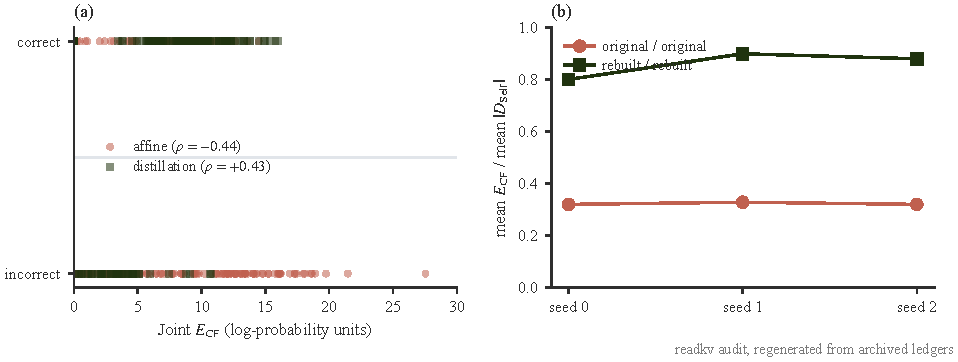
\includegraphics[width=\linewidth]{figures/fig7_ecf.pdf}
\caption{Counterfactual error as a diagnostic. (a) Joint dual correctness against first-token $E_{\mathrm{CF}}$ for all 180 rebuilt-validation pairs per mapper; the rank correlation reverses sign between mappers. (b) Mean $E_{\mathrm{CF}}$ divided by mean $|D_{\mathrm{Self}}|$: the rebuilt cell is not merely a rescaled version of the original one.}
\label{fig:ecf}
\end{figure}

\subsection{Full-candidate scoring retains the direction but changes the magnitude}

\begin{table}[tbp]
\centering
\caption{Scoring follow-up on semantic pairs with distinct candidates and exchanged gold labels. Native/transferred entries are Self/Joint dual-correctness percentages. The final three columns give $L$ in points.}
\label{tab:sequence}
\begin{tabular}{lrrrrrrr}
\toprule
& & & \multicolumn{2}{c}{Native / transferred} & \multicolumn{3}{c}{$L$ (points)}\\
\cmidrule(lr){4-5}\cmidrule(l){6-8}
Cell & Seed & Pairs & First & Full & First & Full & Norm.\\
\midrule
\SequenceRows
\bottomrule
\end{tabular}
\end{table}

\begin{table}[tbp]
\centering
\caption{Version difference $L_{\mathrm{A11}}-L_{\mathrm{A00}}$ under each scoring rule. Values and exploratory template-family intervals are in percentage points.}
\label{tab:sequence-contrast}
\begin{tabular}{rrrr}
\toprule
Seed & First token & Full sequence & Length-normalized\\
\midrule
\MainContrastRows
\bottomrule
\end{tabular}
\end{table}

\begin{figure}[tbp]
\centering
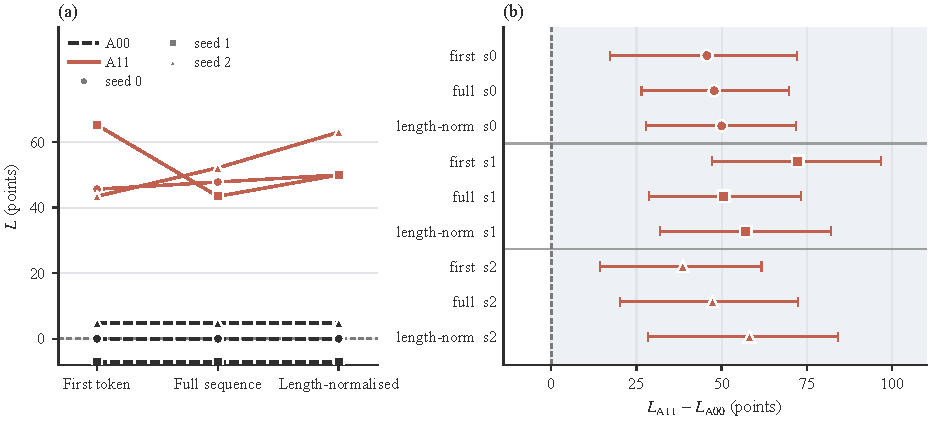
\includegraphics[width=\linewidth]{figures/fig4_scoring.pdf}
\caption{Candidate-score sensitivity on the semantic subset. (a) $L$ under the three readouts for the two diagonal cells. (b) The version contrast $L_{\mathrm{A11}}-L_{\mathrm{A00}}$ with template-family intervals; shading marks positive contrasts. Only the diagonal cells were scored with full sequences.}
\label{fig:scoring}
\end{figure}

We evaluated A00 and A11 using the same scoring procedure in six runs. The main analysis keeps F1--F4 pairs with two distinct candidates and exchanged gold labels, leaving 42/42/41 pairs in A00 and 46 in each A11 seed. All six runs contain separate audit records for every branch. The 2,880 records cover 5,340 forwards. The log checks confirm that the receiver receives the query followed by one candidate prefix token per incremental forward, with consistent position offsets and input fingerprints.

Under full-sequence scoring, A11 retains a gap of 43.5--52.2 points (Table~\ref{tab:sequence}). A11 minus A00 remains positive in all three seeds with either scoring rule, including after length normalization (Table~\ref{tab:sequence-contrast}). The magnitude can change. In seed~1, the A11 gap falls from 65.2 to 43.5 points. Self drops from 87.0\% to 73.9\% while Joint increases from 21.7\% to 30.4\%. The paired difference in $L$ is $-21.7$ points, with an exploratory interval of $[-34.0,-13.0]$. This is evidence of magnitude sensitivity even though the direction persists.

We extended the readout to every F1--F4 pair and then to all 60 validation pairs using the archived per-pair scores (Appendix~\ref{app:sequence}). Dropping the distinct-candidate requirement keeps 46 pairs per cell but still only six template families: F1--F4 themselves contain six families, so the cluster count cannot be raised without including the F5/F6 control slices. Using all 60 pairs gives eight families and the same directional pattern: in seed~1 the A11 gap is $61.7$ points under first-token scoring and $40.0$ under full-sequence scoring, a $21.7$-point reduction matching the main analysis. With eight families the intervals remain exploratory, and no sealed-test score was added. Figure~\ref{fig:scoring} shows both readouts and the resulting version contrast.

\subsection{Behavioral baseline}

We also evaluated a distillation baseline on the reconstructed validation sets. Its mapper was trained for eight epochs with about 7.34 million gradient-optimized parameters to match receiver behavior from its native cache. It uses the same model pair and evaluation data as the affine mapper. Its optimization budget is different. Its Self--Joint drop ranges from 1.7 to 16.7 points over all slices, with a 21.7-point drop in seed~1 when restricted to the four semantic slices. We therefore report smaller observed drops under this baseline and the sensitivity to slice selection (Appendix~\ref{app:factorial}). As the previous section shows, its counterfactual error is not separated from the affine mapper's despite the large correctness difference. Figure~\ref{fig:slices} shows both mappers and the slice-level view of every cell.

\begin{figure}[tbp]
\centering
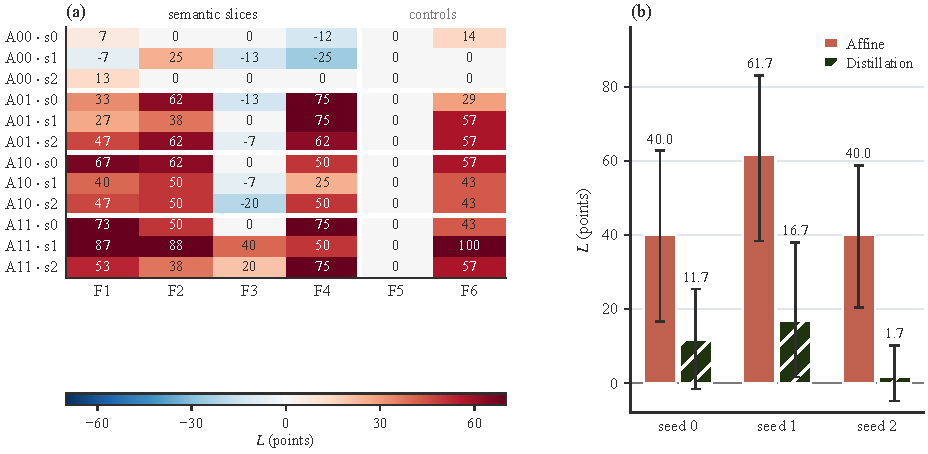
\includegraphics[width=\linewidth]{figures/fig6_slices.pdf}
\caption{Slices and mappers. (a) $L$ in points per slice, cell and seed; F1--F4 are the semantic slices and F5 and F6 are the controls, which are excluded from the direction-consistency analysis. (b) $L$ in points on the rebuilt validation sets for the affine map (solid) and the distillation baseline (hatched), with template-family intervals. The two mappers differ in optimisation budget.}
\label{fig:slices}
\end{figure}

\section{Discussion}

The audit shows what can change when a cache-transfer benchmark is rebuilt. Calibration affects the map itself; validation changes the tasks and the native reference against which it is judged. A positive $L$ change can result from a weaker transferred answer, a stronger native answer, or both. A second score definition distinguishes a pattern tied to a single-token approximation from one whose direction holds under two ways of ranking the same candidates. Here the reconstructed-corpus correctness loss retains its direction, with an appreciable difference in magnitude.

The control and metric checks qualify how the reversal should be read. Joint's counterfactual error is no larger than the mismatched and zero-cache controls, close to the randomized control and significantly smaller than zero-cache in one seed, yet its dual correctness collapses; a pre-declared equivalence test succeeds in only one of three seeds. Counterfactual error therefore cannot stand in for transfer utility. Its scale is not explained by the Self denominator alone, its rank correlation with correctness reverses sign between mappers, and its intervals do not separate two mappers whose correctness differs by tens of points. Reporting native and transferred correctness together, with explicit controls, is more informative than reporting a single discrepancy statistic.

\paragraph{Limitations and next steps.}
The experiment is an audit of one equal-depth model pair and synthetic Chinese template data. Exact effects may vary across pairs, languages, tasks or calibration procedures. Template-family intervals are exploratory because validation has eight families per version and the semantic subset six. The rebuilt corpus changes several properties at once; we have not run the single-defect interventions (de-duplication only, degenerate-pair removal only, entity separation only, template separation only) that would attribute the gap to a specific flaw. The diagonal scoring check covers only A00 and A11; the sealed test, a second model pair such as 4B$\to$1.7B, and a parameter-matched external baseline remain unevaluated. An earlier SQuAD anchor was floor-limited for the native reader and is not used as evidence here. We make no inference about a clean-data mechanism or about whether the original mechanism claim could be recovered. For benchmark audits, these findings support checking corpus splits and labels, reporting native and transferred correctness together, testing against explicit no-information controls, and verifying tie handling and candidate scoring before interpreting a counterfactual gap.

\paragraph{Data and code availability.}
The anonymous supplement contains evaluation-derived numeric ledgers, a CPU replay script and a reproduction guide. It reconstructs the tables, applies a common tie rule, and regenerates the reported intervals and the control tests from archived outputs without requiring weights or accelerators. The original model files were recorded under local snapshot aliases so exact checkpoint contents are outside this replay's verification scope.

\bibliographystyle{tmlr}
\bibliography{references}

\appendix
\setcounter{totalnumber}{5}
\section{Corpus-version contrasts and controls}
\label{app:factorial}

\begin{table}[!htbp]
\centering
\caption{Predefined corpus-version contrasts and the descriptive interaction. Estimates and sample-weighted family intervals are in points. The two cross-validation contrasts independently resample eight clusters per version.}
\begin{tabular}{lrrr}
\toprule
Contrast & Seed 0 & Seed 1 & Seed 2\\
\midrule
\FactorialContrastRows
\bottomrule
\end{tabular}
\end{table}

\begin{table}[!htbp]
\centering
\caption{Equal weight per template family as an alternative estimand for cross-validation comparisons. Both the point and interval use family weighting.}
\begin{tabular}{lrrr}
\toprule
Contrast & Seed 0 & Seed 1 & Seed 2\\
\midrule
\EqualFamilyRows
\bottomrule
\end{tabular}
\end{table}

\begin{table}[!htbp]
\centering
\caption{Affine on reconstructed calibration and validation: first-token Joint $E_{\mathrm{CF}}$ by family and pair resampling, control means, and semantic direction agreement.}
\small
\begin{tabular}{lrrrrrr}
\toprule
Seed & Joint (family) & Joint (pair) & Mismatch & Zero & Random & Agree / eligible\\
\midrule
\AffineControlRows
\bottomrule
\end{tabular}
\end{table}

\begin{table}[!htbp]
\centering
\caption{Control means against Joint on the rebuilt validation sets. Family bootstrap 95\% intervals in log-probability units.}
\begin{tabular}{lrrr}
\toprule
Seed & Control & Mean [95\% CI] & Joint [95\% CI]\\
\midrule
\ControlMeanRows
\bottomrule
\end{tabular}
\end{table}

\begin{table}[!htbp]
\centering
\caption{First-token distillation baseline. Self and Joint are percentages. $L$ intervals and the F1--F4 gap are in percentage points. Error intervals use template-family resampling.}
\small
\begin{tabular}{rrrrrr}
\toprule
Seed & Self & Joint & $L$ [interval] & F1--F4 $L$ & $E_{\mathrm{CF}}$ [interval]\\
\midrule
\KDRows
\bottomrule
\end{tabular}
\end{table}

For A00 the F1--F4 drops are 0.0, $-6.5$ and 4.3 points, whereas the other cells range from 23.9 to 65.2 points under the same slice restriction. Dropping identical candidates gives 2.0, $-6.1$ and 4.2 points for A00 and 28.6--69.8 points for the other cells. The numeric supplement provides per-cell and per-seed F6 results.

\section{Metric validity and mapper separation}
\label{app:metric}

\begin{table}[!htbp]
\centering
\caption{Spearman rank correlation between dual correctness and $E_{\mathrm{CF}}$ on the 180 rebuilt-validation pairs per mapper.}
\label{tab:rank}
\begin{tabular}{lrrr}
\toprule
Mapper & $\rho$ & $p$ & Pairs\\
\midrule
\RankRows
\bottomrule
\end{tabular}
\end{table}

\begin{table}[!htbp]
\centering
\caption{First-token $E_{\mathrm{CF}}$ family intervals and dual correctness for the affine mapper and the distillation baseline on the rebuilt validation sets.}
\begin{tabular}{rrrrr}
\toprule
Seed & Affine $E_{\mathrm{CF}}$ & KD $E_{\mathrm{CF}}$ & Affine dual & KD dual\\
\midrule
\MapperGapRows
\bottomrule
\end{tabular}
\end{table}

\section{Candidate scoring sensitivity}
\label{app:sequence}

\begin{table}[!htbp]
\centering
\caption{Full-minus-first change in $L$ for A11 and in the A11--A00 version contrast. Family-equal estimates and intervals use equal weight per family. All units are percentage points.}
\small
\begin{tabular}{rrrrr}
\toprule
& A11 & \multicolumn{3}{c}{Change in version contrast}\\
\cmidrule(lr){2-2}\cmidrule(l){3-5}
Seed & Family & Family & Pair & Family-equal \\
\midrule
\ScoringChangeRows
\bottomrule
\end{tabular}
\end{table}

\begin{table}[!htbp]
\centering
\caption{Scoring sensitivity using all 60 validation pairs. $L$ values are in percentage points. Identical-candidate controls remain in this comparison.}
\begin{tabular}{lrrrr}
\toprule
Cell & Seed & First token & Full sequence & Length-normalized\\
\midrule
\AllPairsRows
\bottomrule
\end{tabular}
\end{table}

\begin{table}[!htbp]
\centering
\caption{Extended scoring subsets: pair counts and template families per cell and seed. The distinct-candidate subset is the main analysis; F1--F4 and all-60 subsets are sensitivity analyses from archived scores.}
\begin{tabular}{lrrrr}
\toprule
Subset & Cell & Seed & Pairs & Families\\
\midrule
\ScoringCountRows
\bottomrule
\end{tabular}
\end{table}

\begin{table}[!htbp]
\centering
\caption{Extended scoring on all 60 validation pairs (eight template families). $L$ values and family bootstrap intervals are in percentage points.}
\begin{tabular}{lrrrr}
\toprule
Cell & Seed & First token & Full sequence & Length-normalized\\
\midrule
\ExtendedScoringRows
\bottomrule
\end{tabular}
\end{table}

\begin{table}[!htbp]
\centering
\caption{Version contrast $L_{\mathrm{A11}}-L_{\mathrm{A00}}$ on all 60 pairs, with family bootstrap intervals in percentage points.}
\begin{tabular}{rrrr}
\toprule
Seed & First token & Full sequence & Length-normalized\\
\midrule
\ExtendedContrastRows
\bottomrule
\end{tabular}
\end{table}

For an independent boundary check, tokenizing the two strings jointly gave the same query--candidate boundary as concatenating their separate token sequences in all six scoring runs. Within the primary subset neither two candidates with a shared first token nor strict candidate prefixes were observed. Each A11 seed includes seven pairs with unequal candidate lengths. Restricting A11 to the 39 equal-length pairs per seed gives full-sequence $L$ of 48.7, 43.6 and 56.4 points. This equal-length check was added during analysis; the primary comparison and the all-pair comparison above use the same examples within each scoring readout.

\end{document}
